\Chapter{Interação com o avatar}

 Nessa etapa, para construção do ambiente virtual, o software Blender\footnote{Blender - http://www.blender.org/} foi utilizado para modelagem, e para a produção das animações do avatar. A biblioteca PyGame\footnote{PyGame - http://www.pygame.org} foi usada como motor gráfico (engine).

Blender é um software multiplataforma de modelagem, animação, texturização, composição, renderização,
edição de vídeo e criação de aplicações interativas em 3D, como jogos, através de seu
motor de jogo integrado, o Blender Game Engine, inclui suporte a Python como linguagem
script, que pode ser usada tanto no Blender quanto em seu motor de jogo, e possui código aberto.
Ele está sob a licença GNU-GPL, que permite a qualquer pessoa ter acesso ao código-fonte do programa \cite{Blender3D}.

PyGame é um conjunto de módulos em Python projetado para jogos. Permitindo que games e programas de multimidia completos sejam escritos na linguagem Python. É gratuito, portátil, código aberto, não requer OpenGL\footnote{OpenGL (Open Graphics Library) - http://www.opengl.org/} e usa funções otimizadas em C e Assembly para funções essenciais.

Na Figura \ref{img:ambiente_virtual} o avatar (agente que representa o usuário) está no ambiente virtual executando a animação de estado de espera (\textit{default}) enquanto nenhum gesto é reconhecido. O ambiente virtual é definido pela imagem de fundo, pelo avatar e outros objetos que possam futuramente ser inseridos no cenário.

\begin{figure}[!htbp]
  \center
  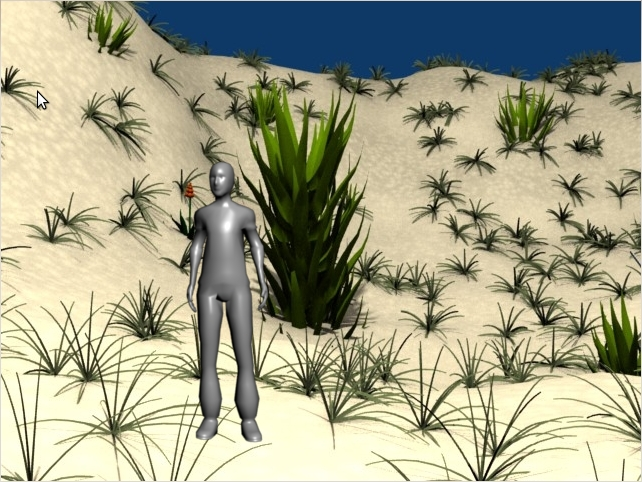
\includegraphics[scale=0.40]{imagens/ambiente_virtual.jpg}
  \caption{Ambiente Virtual.}
  \label{img:ambiente_virtual}
\end{figure}


\section{Criando as animações}

Existem sites que são repositórios online de diversos modelos em 3D, como pessoas, carros, roupas, etc, disponíveis em diferentes formatos de acordo com os vários softwares de modelagem 3D. Blender também possui esses repositórios online, o avatar usado nesse sistema foi baixado de um repositório online gratuito.

Para produzir as animações, é preciso salvar as diferentes poses desses modelos no decorrer dos frames. Nesse sistema a taxa de quadros é trinta, então com a finalidade de evitar incoerências, as animações do avatar também foram gravadas a uma taxa de trinta quadros por segundo.

Os modelos são ligados a um tipo de esqueleto, chamado de \textit{armature}, que dita quais são as articulações do modelo. As rotações e translações das partes do modelos são feitas de acordo com a quantidade e local dos membros do esqueleto. A Figura \ref{img:armature} exibe a posição desse esqueleto nos quadros 1, 15 e 30. Blender automaticamente produz os frames intermediários entre essas poses. Os frames são exportados em imagens no formato PNG\footnote{PNG - Portable Network Graphics}, porque esse formato suporta o canal alfa e isso permite que o fundo possa ser retirado e substituído pelo fundo escolhido para o ambiente virtual.

\begin{figure}[!htbp]
  \centering
  \subfigure[Frame 1]{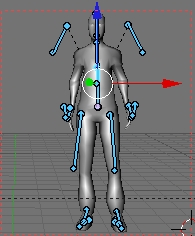
\includegraphics[width=4cm]{imagens/armature_1.jpg}}
  \subfigure[Frame 15]{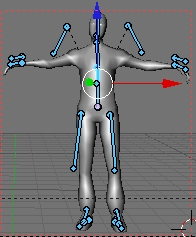
\includegraphics[width=4cm]{imagens/armature_15.jpg}}
  \subfigure[Frame 30]{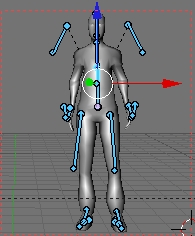
\includegraphics[width=4cm]{imagens/armature_1.jpg}}
  \caption{Posição da armature em frames selecionados.}
  \label{img:armature}
\end{figure}

\section{Criando as interações}

As sequências das animações exportadas pelo Blender são armazenadas para serem utilizadas em tempo real pelo motor gráfico, em nosso sistema o PyGame. As imagens são armazenadas em vetores e a todo momento uma função atualiza na tela a impressão do fundo e do avatar.

Para as animações onde o avatar caminha para a esquerda ou direita, sua posição no ambiente também é alterada, subtraindo-se e adicionando da variável que armazena sua localização no eixo X.

Toda vez que um gesto é reconhecido pelo módulo de identificação, esse gesto é armazenado em uma fila, responsável pela sequência das animações. Ao final de cada animação, o primeiro elemento da fila é retirado dela e executado pelo avatar. Uma variável responsável pelo estado do avatar recebe os valores dessa fila em ordem. Essa estrutura foi utilizada para evitar que a animação atual do avatar fosse interrompida bruscamente caso um gesto novo fosse identificado antes desse animação ter sido concluída.

A Figura \ref{img:animacoes} mostra alguns frames das animações utilizadas para cada um dos gestos no sistema, inclusive a animação executada enquanto nenhum gesto é identificado (default) e a Figura \ref{img:fundo_ambiente_virtual} a imagem de fundo do ambiente virtual, que pode ser substituída por qualquer outra imagem.

\begin{figure}[!htbp]
  \center
  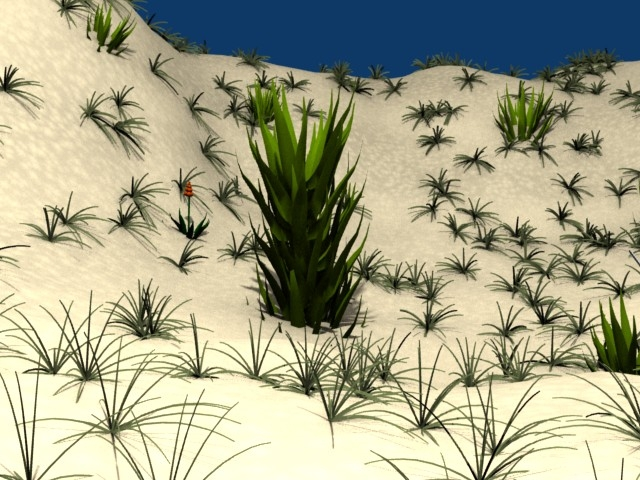
\includegraphics[scale=0.25]{imagens/fundo_ambiente_virtual.jpg}
  \caption{Fundo do Ambiente Virtual.}
  \label{img:fundo_ambiente_virtual}
\end{figure}


\begin{figure}[!htbp]
\center
\begin{tabular}{ccccccc}
\subfigure{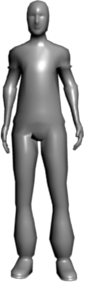
\includegraphics[scale=0.25]{imagens/standing_animation_1.jpg}} & \hspace{0.5cm} &
\subfigure{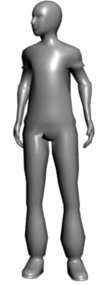
\includegraphics[scale=0.25]{imagens/standing_animation_2.jpg}} & \hspace{0.5cm} &
\subfigure{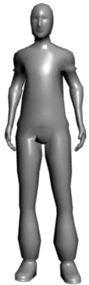
\includegraphics[scale=0.25]{imagens/standing_animation_3.jpg}} & \hspace{0.5cm} &
\subfigure{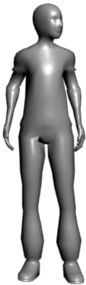
\includegraphics[scale=0.25]{imagens/standing_animation_4.jpg}}
\\

\subfigure{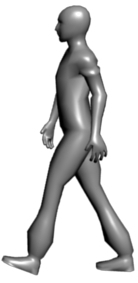
\includegraphics[scale=0.25]{imagens/walk_left_animation_1.jpg}} & &
\subfigure{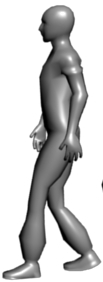
\includegraphics[scale=0.25]{imagens/walk_left_animation_2.jpg}} & &
\subfigure{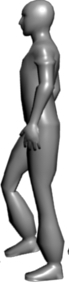
\includegraphics[scale=0.25]{imagens/walk_left_animation_3.jpg}} & &
\subfigure{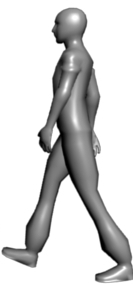
\includegraphics[scale=0.25]{imagens/walk_left_animation_4.jpg}}
\\
\subfigure{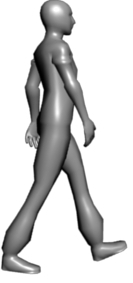
\includegraphics[scale=0.25]{imagens/walk_right_animation_1.jpg}} & &
\subfigure{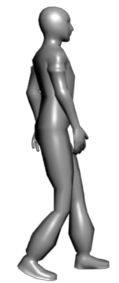
\includegraphics[scale=0.25]{imagens/walk_right_animation_2.jpg}} & &
\subfigure{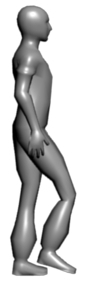
\includegraphics[scale=0.25]{imagens/walk_right_animation_3.jpg}} & &
\subfigure{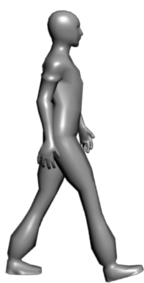
\includegraphics[scale=0.25]{imagens/walk_right_animation_4.jpg}}
\\
\subfigure{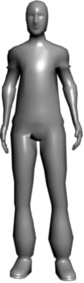
\includegraphics[scale=0.25]{imagens/right_arm_up_animation_1.jpg}} & &
\subfigure{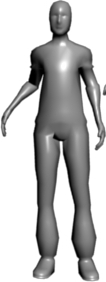
\includegraphics[scale=0.25]{imagens/right_arm_up_animation_2.jpg}} & &
\subfigure{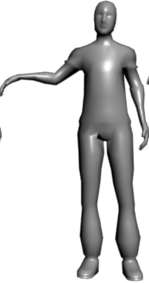
\includegraphics[scale=0.25]{imagens/right_arm_up_animation_3.jpg}} & &
\subfigure{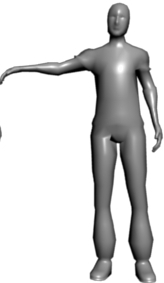
\includegraphics[scale=0.25]{imagens/right_arm_up_animation_4.jpg}}
\\
\subfigure{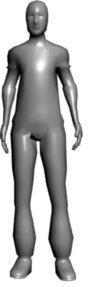
\includegraphics[scale=0.25]{imagens/left_arm_up_animation_1.jpg}} & &
\subfigure{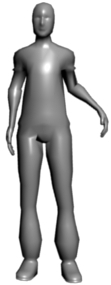
\includegraphics[scale=0.25]{imagens/left_arm_up_animation_2.jpg}} & &
\subfigure{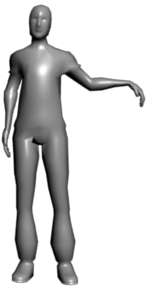
\includegraphics[scale=0.25]{imagens/left_arm_up_animation_3.jpg}} & &
\subfigure{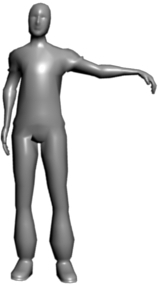
\includegraphics[scale=0.25]{imagens/left_arm_up_animation_4.jpg}}
\\
\subfigure{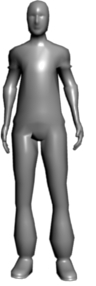
\includegraphics[scale=0.25]{imagens/both_arms_up_animation_1.jpg}} & &
\subfigure{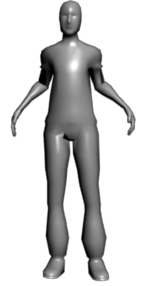
\includegraphics[scale=0.25]{imagens/both_arms_up_animation_2.jpg}} & &
\subfigure{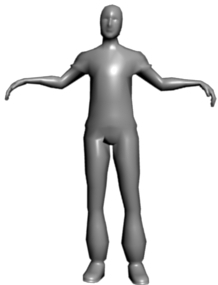
\includegraphics[scale=0.25]{imagens/both_arms_up_animation_3.jpg}} & &
\subfigure{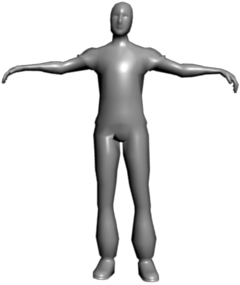
\includegraphics[scale=0.25]{imagens/both_arms_up_animation_4.jpg}}
\end{tabular}
\caption{Frames 1, 5, 10 e 15 das animações criadas para o avatar.}
\label{img:animacoes}
\end{figure}

